\documentclass[prd, showpacs,nofootinbib,amsmath,amssymb,12pt]{revtex4}
\usepackage{amsfonts, amssymb, amsmath, graphicx, comment, bm, slashed}
\usepackage[colorlinks]{hyperref}
\usepackage{dcolumn}
\usepackage{bm}
\usepackage[caption=false]{subfig}
\usepackage{multirow}
\usepackage{mathrsfs,cleveref}
\crefformat{equation}{Eq.~(#2#1#3)}
\crefformat{section}{Sec.~#2#1#3}
\usepackage[numbers,sort&compress]{natbib}

\begin{document}
\title{Magnetized color-flavor locked quark matter and its Bose-Einstein condensed phases in Nambu-Jona-Lasinio model with axial anomaly }
\author{Xiao-bing Zhang$^1$}
\author{Fu-Ping Peng$^1$}
\author{Yun-ben Wu $^1$}
\author{Yi Zhang$^2$}
\affiliation{$^1$School of Physics, Nankai University,\\Tianjin  300071, China}
\affiliation{$^2$ Department of Physics, Shanghai Normal University,\\ Shanghai 200230, China}


\date{\today}
\begin{abstract}
Previous studies show that there exist possible coexistence of diquark and chiral condensates and  critical phenomena in the moderate-density and zero-temperature quark matter,
as long as the QCD axial anomaly is considered.
In the three-flavor Nambu-Jona-Lasinio model with axial anomaly,
we take the influences of rotated electromagnetic field into account and explore the phase structure of  magnetized color-flavor-locked  matter.
Due to the coupling to rotated-charged quarks, the magnetic field is found to facilitate a specific diquark Bose-Einstein condensed phase that referred as $\text{BEC}_\text{I}$.
 With increasing magnetic field, the coexistence phase becomes superseded  by the newly defined $\text{BEC}_\text{I}$ phase gradually 
 and the inverse magnetic catalysis happens for intermediate magnetic fields. For strong fields (say $eB>2.25\times10^{19}$G) , 
 %the $\text{BEC}_\text{I}$ existence
 the complete color-flavor locked symmetry broken
  makes the critical phenomena different from the zero field results   totally.
Also, it is observed that   $\text{BEC}_\text{I}$   occurs at relatively larger quark chemical potential and  relatively weak axial-anomaly coupling, which might be important for  the physics of magnetars.

\end{abstract}
\maketitle

\section{Introduction}
The phases of strongly interacting matter described by quantum chromodynamics (QCD) have attracted great interests for years.
The low-energy ground state of QCD is the hadron phase with condensation of quark-antiquark pairs,
namely the chiral condensate $\langle\bar{q}q\rangle$.
%, and it undergoes transition to the quark-gluon plasma phase at high temperature.
At low temperature and high baryon number density,
the Bardeen-Cooper-Schrieffer (BCS) pairing mechanism among quarks has been proposed and the diquark condensate $\langle qq\rangle$ leads to various color-superconducting phases, see e.g. Refs.~\cite{alford2004dense,alford1998qcd} for reviews.
For three-color and three-flavor quark matter in the chiral limit, the color-superconducting phase corresponds to the color-flavor-locked (CFL)  matter,
which suggests to be the ground state of QCD for very high densities~\cite{alford1998qcd}.
%On account of these phases, many versions of QCD phase diagram were given schematically and,
%in particular, several of QCD critical points were suggested theoretically in literatures.

At intermediate baryon number density, there exists the coexistence (COE) phase with not only chiral condensate as well as diquark condensate under appropriate conditions.
Such kind of critical phenomena was firstly predicted by a Ginzburg-Landau (GL) analysis with the interplay between chiral and
diquark condensates induced by the QCD axial anomaly~\cite{yamamoto2007phase}.
It was further investigated in a phenomenological Nambu-Jona-Lasinio (NJL) model,
where the axial anomaly is taken into account by including the  six-quark effective interactions
caused by instaon effect~\cite{abuki2010nambu}.
%incorporating the interplay between the chiral and diquark condensates induced by
%Due to the chiral-diquark interplay,
%not merely the coexistence (COE) of diquark and chiral condensates but also low-temperature critical phenomena are found to be different from the previous studies.
As detailed in Ref.\cite{abuki2010nambu},
the phenomenon takes place in the sense that the Bose-Einstein condensation (BEC) of diquark ``molecules" emerges firstly
and then a crossover between the diquark BEC phase and the BCS of CFL matter is realized.
Different from high temperature critical phenomena \cite{Shuryak2017Strongly}, critical phenomena in the low-temperature could not be addressed with the first-principle lattice QCD simulations.
Also, its existence is difficult to be observed in experimental heavy ion programs directly.
%The calculations of this critical phenomena are highly model dependent.
%Also, whether the low-temperature critical phenomena exist or not was found to be sensitive to a specific chiral-diquark coupling crucially\cite{}.
%Even for the appropriate model parameters, the given COE region is rather narrow and the obtained critical point is located at the intermediate density\cite{abuki2010nambu}.
%More importantly, the locations of such critical phenomena and their existences are still unclear in reality environment.
% 10.23For instance, if bare quark mass is included, BEC would exclude from the phase diagram and the $2SC_{BEC}$ emerge Ref.~\cite{basler2010role}.
%Also, the effect of confinement was found to relate with Polyakov loop Ref.~\cite{Powell2011Axial}, which indicate the existence of $BEC$.
%In the Ref.[], the local charge-neutrality are not considered.
%Those problem need further discussion.

%On the other hand, the effect of magnetic field in the color superconductor (CSC) matter was studied by many authors~\cite{ferrer2006color,ferrer2007magnetic,ferrer2005magnetic,fukushima2008color,fayazbakhsh2010color,fayazbakhsh2011phase,mandal2013neutrality,mandal2016effect,mandal2017effect}.
In this paper, we will study the influence of magnetic field on  COE phase with chiral and diquark condensate and the critical phenomena.
Our motivations are based on the two folds.
First of all, if  strong magnetic fields could reached the QCD energy scale 
 (say $eB \sim \Lambda_{QCD}^2$ and $\Lambda_{QCD} \simeq$ 200 MeV),  it  would influence QCD phase diagram ( including
the low temperature critical phenomena).
Such a strong field will take magnetic catalysis effect on chiral condensate
$\langle \bar{q}q \rangle$, with increasing  with the magnetic field (the so-called mangetic catalysis (MC)).
Different from the case of low chemical potential, 
for the diquark condensate,  $\langle q q\rangle$,
 a rotated electric charge $\widetilde{Q}$ defined in the color-flavor space,
not a normal electric charge,
 plays the key role. 
 %owing to the rotated electromagnetic mechanism the unbroken symmetry is $U(1)_{\widetilde{Q}}$~\cite{alford1998qcd,alford2000mg}.
 %
Once an unscreened magnetic field $B$ are turned on, some considerable changes have been predicted for the BCS phase.
According to the rotated-charges of quark species, in particular, different magnetic responses lead to the splitting of diquark condensate,
and the correspond color superconducting gaps ~\cite{ferrer2005magnetic,fukushima2008color,ferrer2006color,ferrer2007magnetic}.
When the magnetic energy scale reached to $eB \sim \mu^2$, the distinction between them becomes significant.
However, most of these works were devoted to magnetic effect on the BCS phase of CFL matter, not the BEC  phase in the COE region.
Studying the magnetic effect on the BEC phase   and 
low-temperature phenomena helps to fill vacancies in this area.
    


Secondly and maybe more importantly, it is belived that  there exist strong magnetic fields in the astrophysical "Laboratories",
called as magnetars.
Magnetic fields of the order of $B \sim 10^{14}$ - $10^{15}\text{G}$ can be observed on the surface of Magnetars.
In the interior of compact stars, the strengths can reach $B \sim 10^{18}\text{G}$ and a theoretical upper limit may be up to $B \sim 10^{20}\text{G}$~\cite{lai1991cold}.
On the other hand, it is greatly possible for the core of magnetars to have 
CFL matter.
By the combination of this fact that there exist chiral condensate in the surface of
magnetars, it can be concluded that there may exist the COE phase  in the interface of
magnetars.
Exploring this aspect contributes to the studying for evolution of magnetars and 
validation of model calculations.


%In Ref.\cite{}, an inverse magnetic catalysis for the emergence of diquark BEC phase was found under certain circumstance of magnetic field and the influence on such a BEC-BCS crossover was investigated.
%It is worth to note that the phenomenon around this BEC-BCS crossover is not the above-mentioned critical phenomenon that predicted in three flavor and color QCD system \cite{}.
%For the latter, to the best of our knowledge, the magnetic effect have not yet been elucidated until now.
%Noted that the only place CSC might be observed is the interior region of compact stars, many studies pay attention to the magnetic effect on the CSC  phase.
%For example, the gap splitting are considered when the magnetic field is introduced to BCS phase of CSC.
%It is important and crucial to investigate the relationship between COE, BEC and critical phenomena.
%Since there exist both chiral-condensate and diquark-condensate in COE, the magnetic field influence in expected to be manifold and complicated.
%In NJL-model with axial anomaly in the presence of magnetic effect have not yet been included.
%Exploring this effects is the main purpose of present paper.
%This topic would lay the foundation for the well-resourced phase diagram and possible applications for the physics of magnetars and it is one of the important problems in the context of strongly interacting matter under magnetic fields.

The paper is organized as follow.
In Sec.~\ref{sec:2}, we review  NJL model with axial anomaly  and expand  a kind of NJL model with magnetic field introduced.
%incorporate an applied field $B$ into the NJL model with axial anomaly to study how the chiral-diquark interplay and low-temperature critical point be modified by the presence of magnetic fields.
%Due to the rotated electromagnetic mechanism, there exist the splitting of diquark condensate, namely,
%rotated-charged($\widetilde{Q}$)  and rotated-neutral diquark gaps or channels.
%As magnetic field is introduced, the critical phenomenon changes comparing with zero field resulting.
%The diquark condensates are found to split into the rotated-charged relevant one $s_B$ and the irrelevant one $s$,
%which shares one similarity with the gap splitting in the ``pure" CFL phase without chiral condensate.
%As the consequence, the mean-field thermodynamic potential behaves as the function of three condensates $s_B$,
%$s$ and $\chi$ at the given temperature and quark chemical potential.
%By employing the extended formalism, our attention is first paid to the ${\widetilde{Q}}$-relevant channel of diquark condensate.
%We find that its associated BEC critical point are facilitated significantly by the presence of magnetic fields.
%Then we study how the axial-anomaly induced interplay between chiral and diquark condensates be modified under magnetic fields.
%We find that the interplay itself is facilitated also, which supports the existence of low-temperature critical point totally.
%Our results suggest that this results are caused by the competition of inverse IMC in diquark condensate and MC effect in chiral condensate.
In Sec.~\ref{sec:3} , we give  numerical results in the two typical values of magnetic fields
and plot corresponding order parameters as functions of  chemical potential.
%Compared with the zero-field case,  it was found that  a new defined BEC phase called as  BEC$_\text{I}$ at intermediate value of field,  and so on.
%In Sec.~\ref{sec:3}, 
 We derive the criteria  of diquark Bose-Einstein condensed phases and 
 investigate how the axial anomaly together with magneic field influence the critical phenomenon happened in the COE phase.
%We simplify the criterion condition for BEC$_\text{I}$  in strong field regime and discuss how the strong magnetic fields influence  BEC$_\text{I}$  through the effective diquark coupling or the chiral-diquark coupling constant.

\section{The NJL model of magnetized CFL matter with axial anomaly}
\label{sec:1}

In this section, we firstly review the formalism of NJL model with axial anomaly given in reference\cite{abuki2010nambu}.
And then expand it to the situation with  non-vanishing magnetic fields.
%Finally, we will give the regularization scheme and model parameter.

\subsection{Formalism in the absence of magnetic  field}
\label{sec:2a}
In general, the NJL-type Lagrangian reads
\begin{equation}
	\mathcal{L} = \bar{q} (i\gamma^\mu \partial_\mu + \gamma_0\mu +m_q) q +
	\mathcal{L}^{(4)}+ \mathcal{L}^{(6)},
	\label{eq:lag}
\end{equation}
where $\mu$ is the quark chemical potential, and $m_q$ is the current quark mass.
The four-quark interaction $\mathcal{L}^{(4)}$ consists of $\mathcal{L}^{(4)}_\chi$ and $\mathcal{L}^{(4)}_s$, 
which correspond to the $qq$ and $q\bar{q}$ channel respectively.
The six-quark interaction$\mathcal{L}^{(6)}$ introduce the axial anomaly,
which consists of two parts $\mathcal{L}^{(6)}_{\chi}$ and $\mathcal{L}^{(6)}_{\chi s}$. 
The chiral condensate is defined as 
\begin{equation}
\chi\delta_{ij}= \langle\bar{q}_i q_j\rangle,\quad
\end{equation}
where the indices $(i,j)$ are flavor of quark. 
For three-color and three-flavor QCD, the diquark condensate is defined as \cite{Buballa2002Color}
\begin{equation}
s_{AA'}=\langle q^TC\gamma_5\tau_A\lambda_{A'} q\rangle,
\end{equation}
where $\tau_A$ and $\lambda_{A'}$ denote three antisymmetric Gell-Mann matrices, i.e., $A=2,5,7$.
If we have degenerate light flavors, dense matter is expected to form a so-called color-flavor-locked matter, characterized by the situation $s=s_{22}=s_{55}=s_{77}$.

In the mean-field approximation, the interaction terms in Lagrangian can be written as\cite{abuki2010nambu},  
\begin{equation}
\mathcal{L}^{(4)}_{\chi}=4G\chi\bar{q}q-6G\chi^2, 
\label{eqL4}
\end{equation}	
\begin{equation}
\mathcal{L}^{(4)}_{s}=H[s^*(q^TC\gamma_5\tau_A\lambda_Aq)+h.c.]-3H|s|^2, 
\label{eqL4s}
\end{equation}
\begin{equation}
\mathcal{L}^{\left(6\right)}_{\chi}=-2K\chi^2\bar{q}q+4K\chi^3, 
\label{eqL6chi}
\end{equation}
\begin{equation}
\mathcal{L}^{\left(6\right)}_{\chi s}=-\frac{K'}{4}|s|^2\bar{q}q-\frac{K'}{4}\chi[s^*(q^TC\gamma_5\tau_A\lambda_Aq)+h.c.]+\frac{3K'}{2}|s|^2\chi.
\label{eqL6chis}
\end{equation}
In the four-quark interaction, the couplings for $qq$-channel and $q\bar{q}$-channel are $G$ and $H$ respectively.
$\mathcal{L}^{\left(6\right)}_{\chi}$ is the standard Kobayashi-Maskawa-'t Hooft interaction which couples the chiral condensate only, 
and the interaction coupling is written as $K$.
For the six-quark term $\mathcal{L}^{\left(6\right)}_{\chi s}$ with coupling $K'$, it corresponds to the interplay between chiral and diquark condensates.

Based on the equations above, 
all the $q\bar{q}$-channel interaction terms can be attributed as  the constituent quark mass (the dynamic Dirac mass)
\begin{equation}
M = -4(G-\frac{1}{8}K\chi)\chi + \frac{1}{4}K's^2.
\label{Dmass}
\end{equation}
We ignore the current quark mass $m_q$ all through this work.
The constituent mass is not only made up by four-quark interaction with $G$,
but also related to the axial anomaly, 
manifesting as the Kobayashi-Maskawa-'t Hooft interaction of six-quark interaction $K$ and the chiral-diquark interplay $K'$. 

Similarly, the $qq$-channel  interaction can be given as the color-superconductor gap (the dynamic Majorana mass)
\begin{equation}
\Delta=-2Hs+\frac{1}{2}K'\chi s.
\end{equation}
The coupling $H$ represents the magnitude of diquark attractive interaction.
When the axial anomaly is introduced, it becomes
\begin{equation}
\label{eq:effectivecoupling}
H'=H - \frac{1}{4}K'\chi.
\end{equation}
The additional chiral-diquark interplay $K'$ enhances the diquark attraction. 
This is the reason that the axial anomaly raises the $COE$ of $\langle\bar{q}q\rangle$ , $\langle qq\rangle$ and the diquark BEC phase.
So that the diquark gap is given as $\Delta=-2H's$. 

It is well known that the coupling $H$ represents the magnitude of diquark attractive interaction.
Its appropriate value makes color superconducting becomes possible.
If the axial anomaly is introduced, the effective coupling becomes Eq.~\eqref{eq:effectivecoupling}.
Therefore, the additional chiral-diquark interplay enhance the diquark coupling.
This is the essential reason that the axial anomaly raise the COE of chiral and diquark condensates and thus diquark BEC phase occur
We will investigate this effective coupling with magnetic field in the later section.

In the absence of magnetic field, the thermodynamic potential is written as 
\begin{equation}
\Omega=\Omega_q+U(\chi,s).
\label{eq:1loopu}
\end{equation}
By using the Nambu-Gor'kov formalism,  
the one-loop contribution given as\cite{abuki2010nambu},
\begin{equation}
\Omega_q=-8\sum_{\pm}\int\frac{d^3p}{(2\pi)^3}|\epsilon^8|
-\sum_{\pm}\int\frac{d^3p}{(2\pi)^3}|\epsilon^1|,
\label{oneloopinzero}
\end{equation}
where the singlet and octet represent the ...The sum indices  $\pm$ represent the quasiparticle and anti-quasiparticle excitations respectively. 
In reference\cite{abuki2010nambu}, the renormalization parameter $\Lambda$ is  cut-off for integral. 
The dispersion relation in singlet and octet representations read
\begin{equation}
\epsilon^1=\sqrt{(E\pm\mu)^2+(2\Delta)^2},\quad
\epsilon^8=\sqrt{(E\pm\mu)^2+\Delta^2},
\label{despersionzerofield}
\end{equation}
with the single-particle energy $E=\sqrt{p^2+M^2}$ .

The interaction potential $U$ can be derived from Eqs.(\ref{eqL4} -\ref{eqL6chis}),  which reads\cite{abuki2010nambu}
\begin{equation}
U(\chi,s) = 6G\chi^2 - 4K\chi^3 + 3(H-\frac{K'}{2}\chi)s^2.
\label{potentialterm}
\end{equation}

\subsection{Formalism in the presence of magnetic field}
When the magnetic field is introduced in the CFL matter, the most important physics is the rotated-electromagnetic mechanism\cite{alford1998qcd}, which would redefine the diquark condensate.
This mechanism namely the unbroken symmetry is described by the subgroup $U(1)_{\widetilde{Q}}$,
with $\widetilde{Q}=Q\times\bm{1}+\bm{1}\times T_8/\sqrt{3}$, 
where $Q=\text{diag}(-\frac{1}{3},-\frac{1}{3},\frac{2}{3})$ for $(s,d,u)$ and $T_8=\text{diag}(-\frac{1}{\sqrt{3}},-\frac{1}{\sqrt{3}},\frac{2}{\sqrt{3}})$ for $(b,g,r)$.
And the rotated magnetic field becomes linear combination of an usual photon and the eighth gluon fields. 
Once the magnetic field is switched on, the structure of diquark condensate is changed.
The condensate not only have color-antitriplet, flavor-antitriplet condensate but also the a color-sextet, flavor sextet condensate\cite{ferrer2006Color}.
As the discussion in reference \cite{fukushima2008Color}, we usually ignore the sextet condensate. 
Now we ansatz that the $s=s_{22}$ and $s_B=s_{55}=s_{77}$.
However, the structure of diquark is more then complicate that 
According to the $\widetilde{Q}$ properties of quarks, there actually exist the threes types of pairing patterns:
the neutral, charged and mixed pairings as summarized in Table \ref{tab:1}.\cite{ferrer2005magnetic}.

\begin{table}[ht]
  \caption{classification of pairings, gaps and dispersion relations}
  \centering
   \begin{tabular}{c|c|c|c|c}
    \hline\hline
    Paring  type           & neutral               & mixed                         & \multicolumn{2}{c}{charged}\\
    \hline
    Quark                  & bd\quad gs            & ru\quad gd\quad bs            & rs\quad bu  & gu\quad rd\\
    \hline
    $\widetilde{Q}$        & 0\quad 0              & 0\quad 0\quad 0               & +1\quad -1  & -1\quad +1\\
    \hline
    Diquark condensate     & $s$                   & $s$\quad $s_B$                & \multicolumn{2}{c}{$s_B$}\\
    \hline
    Gap                    & $\Delta$              & $\Delta_1,\Delta_2$           & \multicolumn{2}{c}{$\Delta_B$}\\
    \hline
    Dispersion relation    & $\epsilon^n$          & $\epsilon^m_1,\epsilon^m_2$   & \multicolumn{2}{c}{$\epsilon^c$}\\
    \hline\hline
   \end{tabular}
   \label{tab:1}
\end{table}

For the neutral type ( $bd-gs$ pairing), only the diquark condensate $s$ is involved and the color superconductor gap is determined by it.
In the NJL-model with axial anomaly, the gap reads
\begin{equation}
\Delta=-2H's.
\end{equation}
Correspondingly, the dispersion relation  has the form like 
\begin{equation}
\label{eq:disperzero}
\epsilon^n=\sqrt{(E\pm\mu)^2+\Delta^2},
\end{equation}
for the quark and anti-quark excitations respectively.
In Eq.\eqref{eq:disperzero}, the single particle energy is still $E=\sqrt{p^2+M^2}$ , although the quark mass in Eq.~\eqref{Dmass} needs to be modified(see below).
The neutral pairing contributes one-loop thermodynamic potential
\begin{equation}
\Omega^n_q=-6\sum_{\pm}\int h_{\Lambda}\frac{d^3p}{(2\pi)^3} |\epsilon^n|,
\label{omegaq}
\end{equation}
where the smooth regulator function $h_\Lambda$ has replaced the cut-off regulator scheme in Eq.(\ref{oneloopinzero}).

For the charged type, the paired quarks carry the non-zero rotated charges (the $rs-bu$ and/or $gu-rd$ pairing, see Table \ref{tab:1}).
The gap is determined by the diquark condensate $s_B$,
\begin{equation}
\Delta_B=-2H's_B.
\end{equation}
In this case, the single -particle energy spectrum becomes
\begin{equation}
\label{eq:energyb}
E_B=\sqrt{p^2_3+M^2 + 2neB},
\end{equation}
where $p_3$ is the third component of momentum space, and $n$ is Landau level index($n=0,1,2,...$).
The dispersion relations reads
\begin{equation}
    \epsilon^c=\sqrt{(E_B\pm\mu)^2+\Delta_B^2},
\end{equation}
where the gap $\Delta_B=-2H' s_B$.
By using the substitution:
\begin{equation}
2\int\frac{d^3p}{(2\pi)^3}\rightarrow\frac{eB}{8\pi^2}\sum^{\infty}_n(2-\delta_{n0})\int^{+\infty}_{-\infty} dp_3,
\label{eq:momentumsub}
\end{equation}
one can derive the thermodynamic potential contribution from charged quarks.
For the given cut-off parameter $\Lambda$, we introduce the number of completely occupied Landau levels $n_{max}$, 
\begin{equation}\label{eq:nmax}
  n_{max}= \text{Int}[\frac{\Lambda^2}{2eB}],
\end{equation}
and obtain the one-loop thermodynamic potential 
\begin{equation}
\Omega^c_q=-8\sum_{\pm}\frac{eB}{8\pi^2}\sum_{n=0}^{n_{max}} (2 -\delta_{n0}) \int h^n_{\Lambda,B} dp_3|\epsilon^c|, 
\end{equation}
where $h^n_{\Lambda,B}$ is smooth regularization function for the charged pairing. Together with $h_\Lambda$ , they will be discussed in the following section.

For the mixed type(i.e. $ru-gd-bs$ pairing),  both $s$ and $s_B$ play their roles.
As detailed in Ref.\cite{ferrer2006color,noronha2007color},
the color-superconductor gaps behave as the combination of $\Delta$ and $\Delta_B$,
\begin{equation}
\Delta_{1}=\frac{1}{2}(\sqrt{\Delta^2 + 8\Delta_B^2} + \Delta),\quad
\Delta_{2}=\frac{1}{2}(\sqrt{\Delta^2 + 8\Delta_B^2} - \Delta).
\end{equation}
And the dispersion relation given as
\begin{equation}
\epsilon^m_1=\sqrt{(E\pm\mu)^2+\Delta_1},\quad \epsilon^m_2=\sqrt{(E\pm\mu)^2+\Delta_2}
\end{equation}
Since only neutral quarks are included  in the mixed pairing, 
the thermodynamic potential contribution reads \cite{noronha2007color}
\begin{equation}
\Omega^m_q=-2\sum_{\pm}\int h_{\Lambda}\frac{d^3p}{(2\pi)^3}  \epsilon^m_1 -2\sum_{\pm}\int h_{\Lambda}\frac{d^3p}{(2\pi)^3}  \epsilon^m_2.
\end{equation}

Now we turn to investigate the constituent  mass in the magnetized CFL matter.
Recalling that it stems the interacting terms in the $\bar{q}q$ channel, which is irrelevant to
$qq$ channel. $M$ has the similar form as Eq.(\ref{Dmass}), as long as the  splitting of
diquark condensate is taken into account.
While the first term in R.H.S. of  Eq.(\ref{Dmass}) 
holds unchanged, the splitting  changes the second term of Eq.(\ref{Dmass})
through the chiral-diquark coupling $K'$.
Due to  a simple relation $s^2_{22}+s^2_{55}+s^2_{77} = s^2 + 2s_B^2$ , 
the zero-field result $s^2$ should be replaced  $\frac{1}{3}s^2+\frac{2}{3}s^2_{B}$
in the presence of magnetic field.
Thus Eq.(\ref{Dmass}) in the zero-field result is rewritten as
\begin{equation}
M=-4(G-\frac{1}{8}K\chi)\chi+\frac{1}{12}K's^2+\frac{1}{6}K's^2_B,
\end{equation}
The constituent quark mass can be derived form the Nambu-Gor'kov formalism, and then contribution term of the constituent quark mass comes form the diagonal of the inverse propagator, while the off-diagonal term effect  the quark splitting\cite{abuki2010nambu}.
Thus thus the gap splitting have no influence to the formalism of constituent quark mass.  
Following the same procedure, the interaction potential term Eq.~\eqref{potentialterm} is given by
\begin{equation}
U(\chi,s,s_B)=6G\chi^2-4K\chi^3+(H-\frac{K'}{2}\chi)(s^2+2s^2_B).
\end{equation}
Instead of Eq.~\eqref{eq:1loopu}, the  total thermodynamic potential is the function of 
\begin{equation}
\label{finaleq}
\Omega(\chi,s,s_B)=\Omega^n_q+\Omega^m_q+\Omega^c_q+U.
\end{equation}
In Eq.~\eqref{finaleq}, the contribution from electromagnetic field (say, $\frac{1}{2}B^2$) in this equation has been dropped out, since the magnetic filed penetrate the CFL quark matter freely \cite{ferrer2005magnetic,  ferrer2006color,  ferrer2007magnetic}. 


\subsection{Model parameters and Regularization scheme}
\label{sec:2c}
In the case of non-zero magnetic field, it is well know that the hard cutoff scheme is not suitable. 
Several smooth regulator scheme have been given in literature.
For example, Wood-Saxon-type\cite{fayazbakhsh2010color}, magnetic field independent regularization\cite{allen2015magnetized}, Gaussian-type\cite{noronha2007color} reads
\begin{equation}
h_\Lambda = exp(-p^2/\Lambda^2) 
\end{quation}
and Lorentzian type\cite{Frasca2011Magnetic} reads
\begin{equation}
    h_{\Lambda} = [1+(\frac{p}{\Lambda})^N]^{-1}
\end{equation}
have been introduced.
In our work we follow the Lorentzian type and the momentum space should be Landua level space,
\begin{equation}\label{eq:regulator}
  h_{\Lambda} = [1+(\frac{p}{\Lambda})^N]^{-1}, \quad  h^n_{\Lambda,B}=[1+(\frac{\sqrt{p_3^2 + 2neB}}{\Lambda})^N]^{-1}.
\end{equation}
where $n$ is quantum number and $N$ is the parameter of the smooth regulation factor.
In Fig.\ref{f1} the numerical calculations of constituent quark in low density region shows that the Lorentzian type for $N=5$ is better to improve the unphysical oscillation, compared with Lorentzian $N=15$ and Gaussian-type.

\begin{figure}[ht]
	\centering
	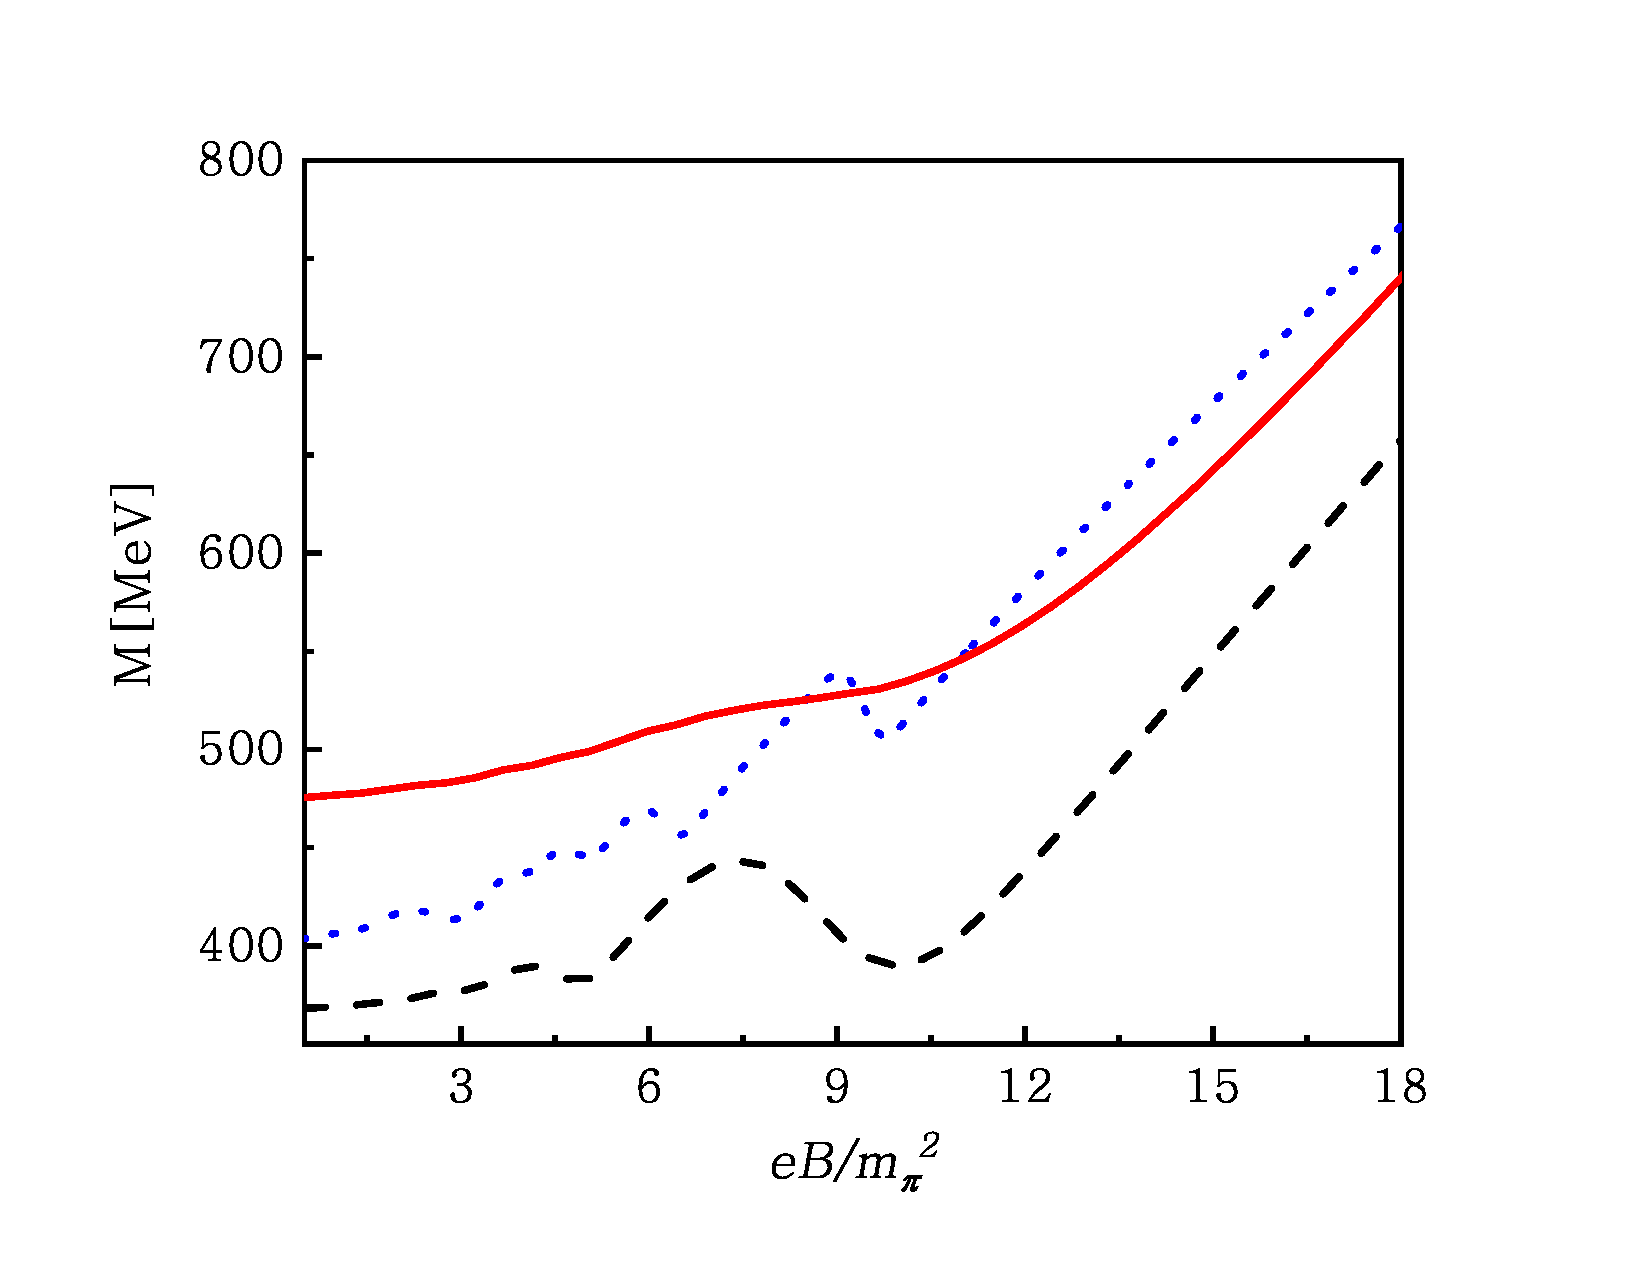
\includegraphics[scale=0.3]{compare.eps}
	\caption{The Lorentzian type where $N=5$ (red sold line) and $N=15$ (cross-line). The Gaussian-like from in blue dotted line.}
	\label{f1}
\end{figure}

%To this end, it should be stressed that van Alphen-de Haas(vA-dH) oscillation happened in gaps (including $\Delta$, $\Delta_B$ and $M$) still exist.
%Recent study suggested a new regulator scheme named "Magnetic Field Independent Regularization"\cite{allen2015magnetized}.
%In Ref.\cite{allen2015magnetized}, the NJL-type model is investigated by using this regularization procedure in which the contributions that are explicitly dependent on the magnetic field turn out to be finite and do not required to be regularized. 

As for the model parameter $G, H, K',K$ and $\Lambda$, 
the momentum cutoff $\Lambda$ and the chiral coupling constant $G$ is fixed by fitting the pion properties in vacuum, e.g.,
the pion mass $m_\pi = 140 MeV$ and the constituent quark $M = 340 MeV$.
The diquark coupling constant $H$ is fixed by fitting the scalar diquark mass.
For the six-fermion coupling constants $K$ and $K'$, one appropriate value of  $K'/K$ maintains to make the low-temperature critical phenomena.
In the present work, we adopt the parameters of Table $I$ ($m_q=0$) in Ref.\cite{abuki2010nambu}.

\section{Numerical calculations and discussions}

Different from the zero-field case, our work exist three order parameter $s$, $s_B$ and $M$.
To determine the 3 gap equation self-consistently, we global minimize $\Omega$ with respect to three order parameter,
\begin{equation}
\frac{\partial\Omega}{\partial s} =0,\quad 
\frac{\partial\Omega}{\partial s_B} =0,\quad 
\frac{\partial\Omega}{\partial \chi} =0.
\end{equation}

\subsection{COE phase region and critical phenomena}
\label{sec:3a}
Theoretically, there should exit different diquark Bose-Einstein-condensate phase distinguished by two diquark condensate $s$ and $s_B$.
Before we introducing the phase diagram, three special phase should be clearly difined.
We refer the diquark Bose-Einstein-condensate phase with $s=0, s_B\neq 0, \chi \neq 0$ as $BEC_\text{I}$ phase. The phase with $s\neq 0, s_B = 0, \chi \neq 0$ as $BEC_\text{II}$ phase. Besides, the BEC phase is defined as $s \neq 0, s_B \neq 0, \chi \neq 0$.

\begin{figure}[ht]
	\centering
	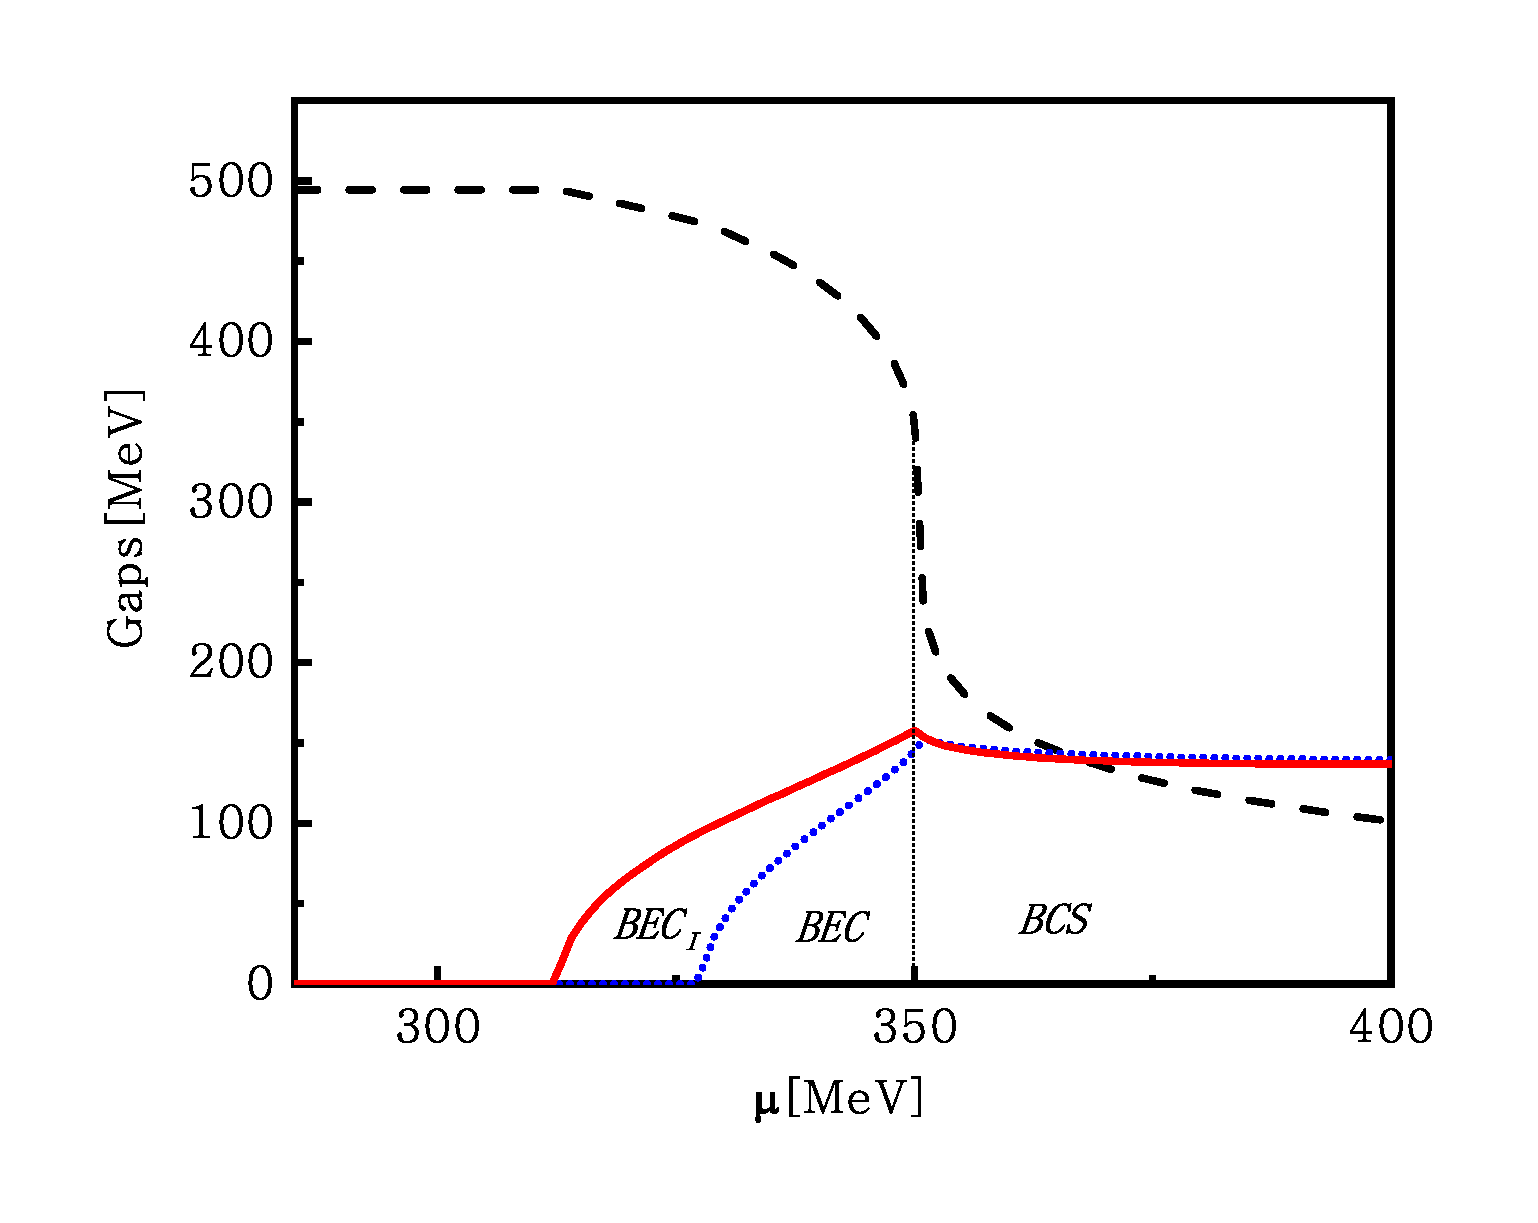
\includegraphics[scale=0.3]{1.eps}
	\caption{The constituent quark mass $M$(dashed-line), and color-superconductor gaps for diquark condensate $\Delta$(red solid line) and $\Delta_B$(blue dotted line) as functions of $\mu$ under the magnetic field value $eB/m^2_\pi=4.6$.}
	\label{f2}
\end{figure}

By using the given model parameters, we calculate the non-zero but weak magnetic field.
This typical results of $COE$ phase region given at $eB=4.6m^2_\pi$ 
%1.40\times10^{19}G.
In Fig.\ref{f2}, at around quark chemical $\mu_c^I=313Mev$, $BEC_\text{I}$ phase appears where the $\Delta$ are allowed equals to zero.
When the $\mu > 327MeV$, the usual $BEC$ phase occurs.
As the $\mu$ keep rising, BEC-BCS crossover happens at $\mu=\mu_X=350MeV$, 
where $\mu_X$ is determined by the crossover condition $M=\mu$. 
Furthermore, the value of constitent quark mass is little larger then calculation in Ref.\cite{abuki2010nambu}, which influenced by the smooth regularization factor we choose.

For weak magnetic case, Fig.\ref{f2} basically same to then zero-field case.
And the critical phenomena also exist and reflect in the continuous behavior of $M$. 
However, the different happend in the region $\mu^I_c<\mu<\mu_X$, that a new phase $BEC_\text{I}$ occurs before $BEC$ phase.

With increasing magnetic filed, $COE$ phase structure and critical phenomena would have remarkable change.
Numerical result shows that the $BEC_\text{I}$ would gradually occupies the $COE$ region and the $BEC$ phase would be suppressed with the increasing $eB$.
Moreover, there exit a threshold value when $BEC$ phase is totally removed by magnetic field.
In Fig.\ref{f3} we give the result of $eB = 9.2m^2_\pi$ greater than the threshold value.
At $\mu=\mu_X=338MeV$, the constituent mass $M$ dramatically decreases.
For chiral phase transition, it actually turn into a first order phase transition, which different from the weak-field(and zero-field) result.
In other words, the critical phenomena at around $\mu_X$ no longer appears unless the axial anomaly reinforce.

\begin{figure}[ht]
	\centering
	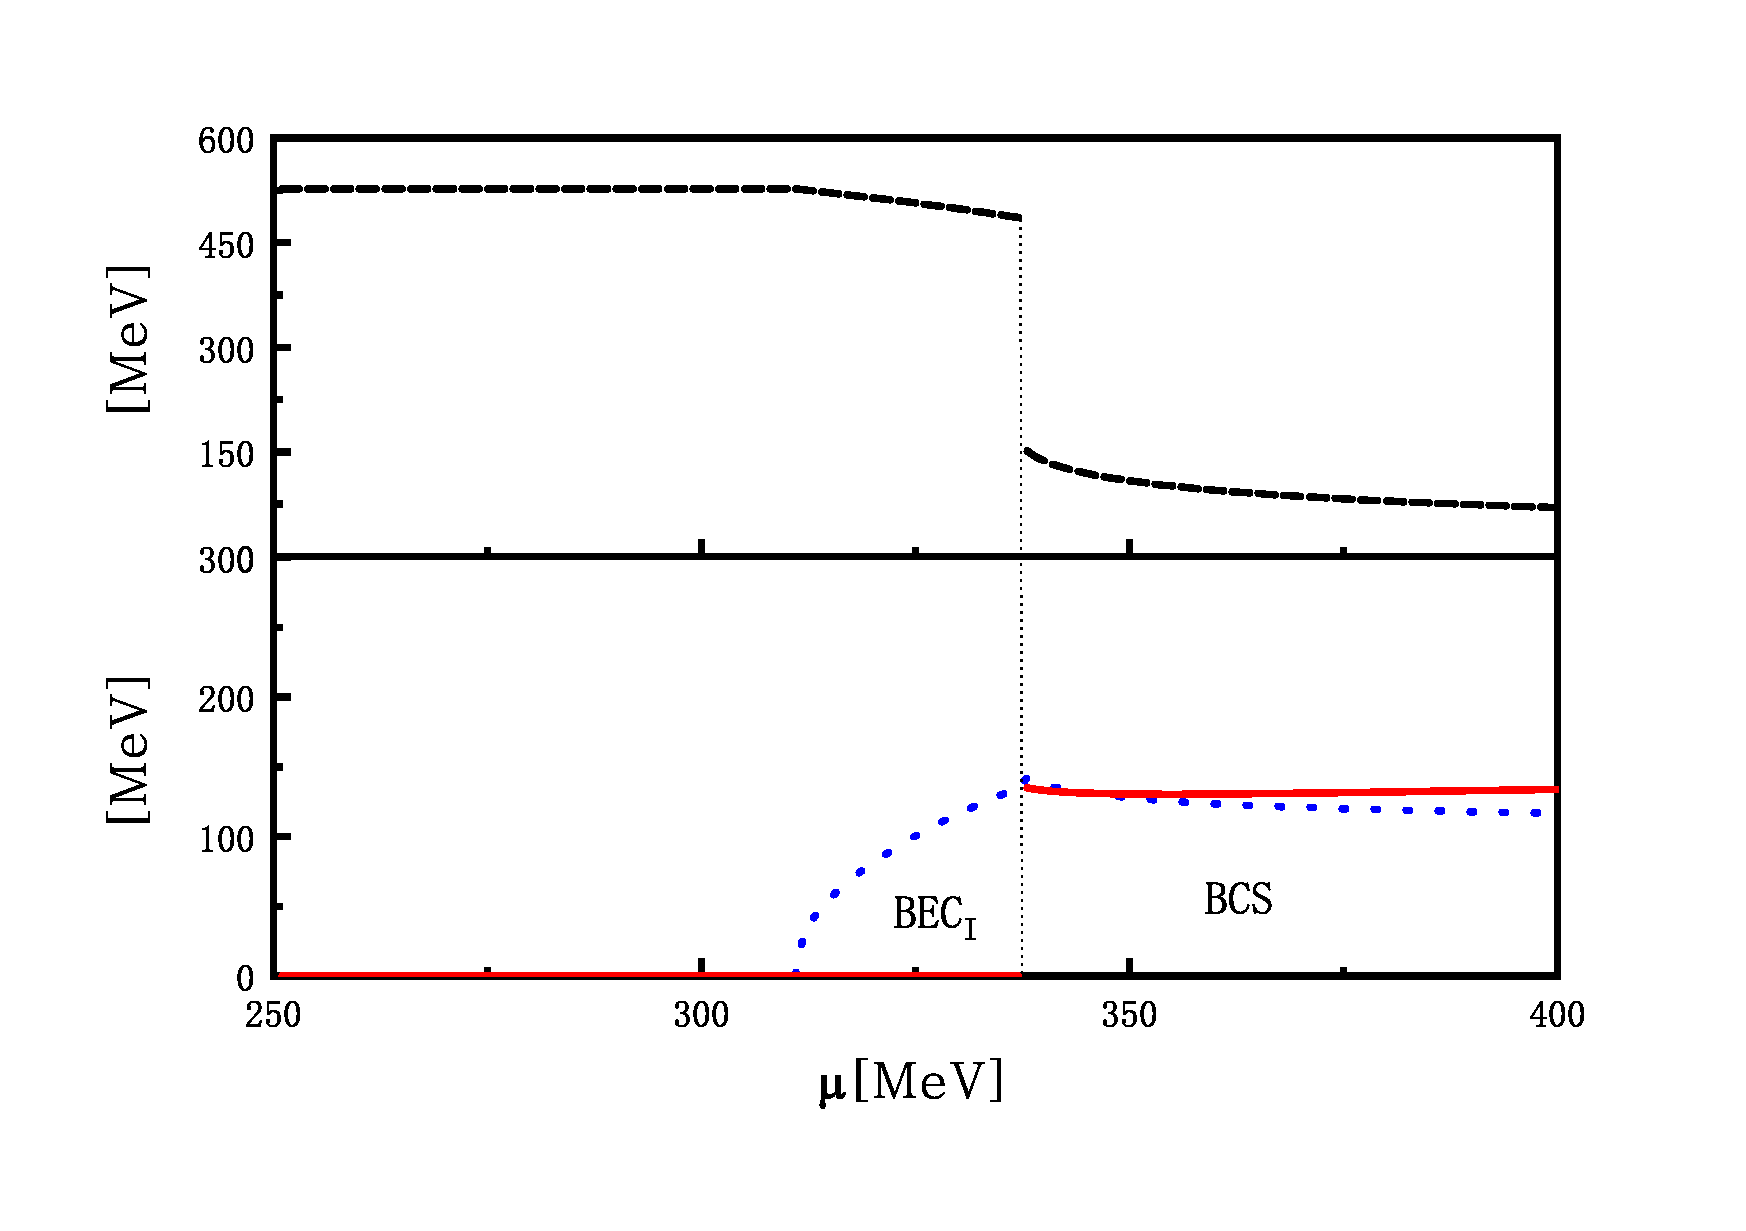
\includegraphics[scale=0.3]{92v2.eps}
	\caption{Similar as Fig.\ref{f2}, but for magnetic filed $eB/m^2_\pi$ equals to $9.2$.}
	\label{f3}
\end{figure}

Introducing magnetic field has changed the COE phase structure and the critical phenomena previously predicted in Ref.\cite{abuki2010nambu}.
Physically, it might be related with the magnetic field induced violation of color-flavor-locked symmetry pattern.
For weak field, only slight violation happened in CFL symmetry. 
The splitting of diquark condensate leads to the separation of $COE$, i.e. $BEC_\text{I}$ and $BEC$.
In this case, critical phenomena have no essential difference from that of zero-field case.
For larger magnitude of magnetic field, the symmetry broken more manifestly.
Because of the enhancing magnetic effects on $BEC_\text{I}$ occurrence (see Sec.4B for detials), only $BEC_\text{I}$ survive in $COE$ region.
Since the $BEC$ phase with $s_B\neq 0$ and $s\neq 0$ there no longer exist the "continuity" between low density chiral broken phase and high density $CFL$ phase.
Even though the axial anomaly interplay is introduced, the critial phenomena predicted in zero-field is hard to achieve.

\subsection{Critical chemical potentials for different BEC occurrences}
\label{sec:3b}
In order to further understand the phase structure obtained in Sec.\ref{sec:3a}, our attention is paid to the criteria  of diquark Bose-Einstein condensed phases.
As a second-order transition,  occurrence of a designated BEC phase can be determined by the Thouless criterion\cite{nishida2005bcs}, i.e.,
%Now we try to explain the critical phenomena by investigating the criterion condition for the occurrence of  BEC phases.
%Considering the second order fluctuations around diquark gaps determined the mean-field approximation,
%the BEC criterion condition have been derived as \cite{Nishida2005BCS}
\begin{equation}
\label{eq:omegasecond}
 \frac{1}{H'}= Q(\vec{q} =0, \omega =0),
\end{equation}
where $H'$ is effective diquark coupling and $Q(\vec{q},\omega)$ is diquark polarization function and can be derived from the usual
quark propagator at one-loop level\cite{nishida2005bcs}.

%where $Q_i$ is the  one-loop quark-quark polarization function and $i$ represents the diquark pairing .

% with the  quark fermion propagator $G_0(\vec{p}, 0) = [\slashed{p}+\mu\gamma_0 - M]^{-1} $.
%Since the occurence of BEC  can be treated as  a second-order phase transition for the corresponding diquark gaps,
%the second-order coefficient being zero determines the critical chemical potential for the BEC phase, i.e.,
%\begin{equation}
%\label{eq:bdiquark}
%	\alpha_2 \sim \frac{1}{H'} - Q_A(\vec{q} = \vec{0},\omega =0) =0.
%\end{equation}
%%This is just the Thouless criterion\cite{Nishida2005BCS} that widely used in condensed matter physics.
%The one-loop quark-quark polarization function  $Q_A$ in Eq.~\eqref{eq:omegasecond} can be archived by
%\begin{equation}
%\label{eq:qqpol}
%Q_A(\vec{q})
%= 2i\int \frac{d^4\vec{p}}{(2\pi)^4}
%\times \text{Tr}[i\gamma_5G_0(\vec{q}-\vec{p})i\gamma_5 C G_0(\vec{p})],
%\end{equation}
%with the  quark fermion propagator $G_0(\vec{p}, 0) = [\slashed{p}+\mu\gamma_0 - M]^{-1} $.
In the absence of magnetic field, the 
polarization function is easily obtained and the  BEC occurrence is determined by
\cite{abuki2010nambu},
\begin{equation}\label{eq:criticalfor0}
  \frac{1}{4H'} =  4\sum_{\pm}\int \frac{d^3p}{(2\pi)^3} \frac{1-2f(E\pm \mu)}{2(E \pm \mu)}dp ,
\end{equation}
where $f(\epsilon) =1/(e^{\epsilon/T} +1)$ is the Fermi distribution function.
At zero temperature,  Eq.~\eqref{eq:criticalfor0} has  the form
\begin{equation}
\label{eq:criticalfor1}
\frac{1}{H'} = \frac{8}{ \pi^2} \int_0^\Lambda\frac{ E p^2}{E^2 - \mu^2} dp,
\end{equation}
where $E$ is the single particle energy and the  hard cut off regulator scheme is included. 

Once the magnetic field is introduced,   the splitting of diquark condensate leads to  Bose Einstein Condensed structure more complicated.
% Different from the BEC phase with non-vanishing $s$ and $s_B$, here we has defined the condensed phase with  $s\neq 0$, $s_B=0$ as
%  $\text{BEC}_\text{I}$ in Sec.\ref{sec:3a} . Besides,  the phase with $s\neq 0$, $s_B=0$ and $\chi  \neq 0$
%  is theoretically possible,  which is referred as  $\text{BEC}_\text{II}$.
Let's firstly consider  the criterion of  $\text{BEC}_\text{II}$  occurrence.
%the diquark condensate in the order parameter is $s$.
The  quarks involved in   $\text{BEC}_\text{II}$  are always neutral.
And thus there is no  direct coupling to magnetic field exists. By using Eq.~\eqref{eq:omegasecond}, 
the $\text{BEC}_\text{II}$ occurrence can be derived as
\begin{equation}
\label{eq:criticalforn}
\frac{1}{H'} =\frac{8}{ \pi^2} \int h_\Lambda  \frac{ E p^2}{E^2 - \mu^2} dp,
\end{equation}
%Compared with Eq.~\eqref{eq:criticalfor0}, the criterion equation of $\text{BEC}_\text{II}$ is formally equivalent with that obtained in the case of $B = 0$,
%excepted that we have introduced 
Eq.~\eqref{eq:criticalforn} has the similar form as Eq.~\eqref{eq:criticalfor1}, except for the smooth regulator function $h_\Lambda$ is introduced in the presence of magnetic field.

For the $\text{BEC}_\text{I}$ occurrence, the  diquark ``molecules"  are associated with the order parameter $s_B$.
As shown in Table.\ref{tab:1}, there exist rotated-charged pairing and the  neutral pairing (the mixed pairing).
For the former,  the single particle  
 for the rotated-charged quarks should be replaced by Eq.~\eqref{eq:energyb}.
%$G_0(\vec{p},0) = [\slashed{p}_{\pm}+\mu\gamma_0 - M]^{-1}$, with $p_{(\pm )} = (p_0,0,\pm\sqrt{2eBn},p_3)$ in Landau gauge.
Also the momentum integral  and the regulator function should be replaced by Eq.~\eqref{eq:momentumsub} and ``Lorenzian type" respectively. 
By taking into account the contributions from both charged and mixed pairing, then the $\text{BEC}_\text{I}$ occurrence becomes
\begin{equation}
\label{eq:criticalforq}
\frac{1}{H'}  =
 \frac{eB}{2\pi^2} \int \sum_{n=0}^{n_{max}} (1 -\frac{\delta_{n0}}{2}) h_{\Lambda, B}^n
\frac{E_B}{E_B^2 -\mu^2 } dp_3 + \frac{4}{ \pi^2} \int  h_{\Lambda}
\frac{Ep^2 }{E^2 - \mu^2} dp.
\end{equation}
In the  first term of R.H.S, the magnetic coupling  has been introduced by the Landau level. 
%that reflects the direct coupling of  rotated-charged quarks to magnetic field.
In the zero-field limit,
 the form of \cref{eq:criticalforq}  is recovered to the known result Eq.~\eqref{eq:criticalfor0} .
 In fact,   the critical condition can be derived alternatively. 
 As a second order transition, it can be general given by using a Ginzburg-Landau
 expansion on the  thermodynamic potential with respect to $\Delta$ and 
$\Delta_B$ , i.e., 
\begin{equation}
  \frac{\partial^2\Omega(\Delta,\Delta_B)}{\partial \Delta^2}|_{\Delta_B =0,\Delta =0} =0 ,\frac{\partial^2\Omega(\Delta,\Delta_B)}{\partial \Delta_{B}^2}|_{\Delta_B =0,\Delta =0} =0.
\end{equation}


%Based on \cref{eq:criticalforn,eq:criticalforq}, we can achieve the critical chemical potentials for $\text{BEC}_\text{I}$ and $\text{BEC}_\text{II}$ occurrence  respectively.
\begin{figure}[h]
  \caption{Critical  values  $\mu_c^\text{I}$  (solid line),     $\mu_c^\text{II}$ ( dashed line)   and  the critical chemical potential $\mu_c$ for BEC  (dashed dotted line)  and the reference 
  chemical potential $\mu_X$ (dotted line)}
  \centering
    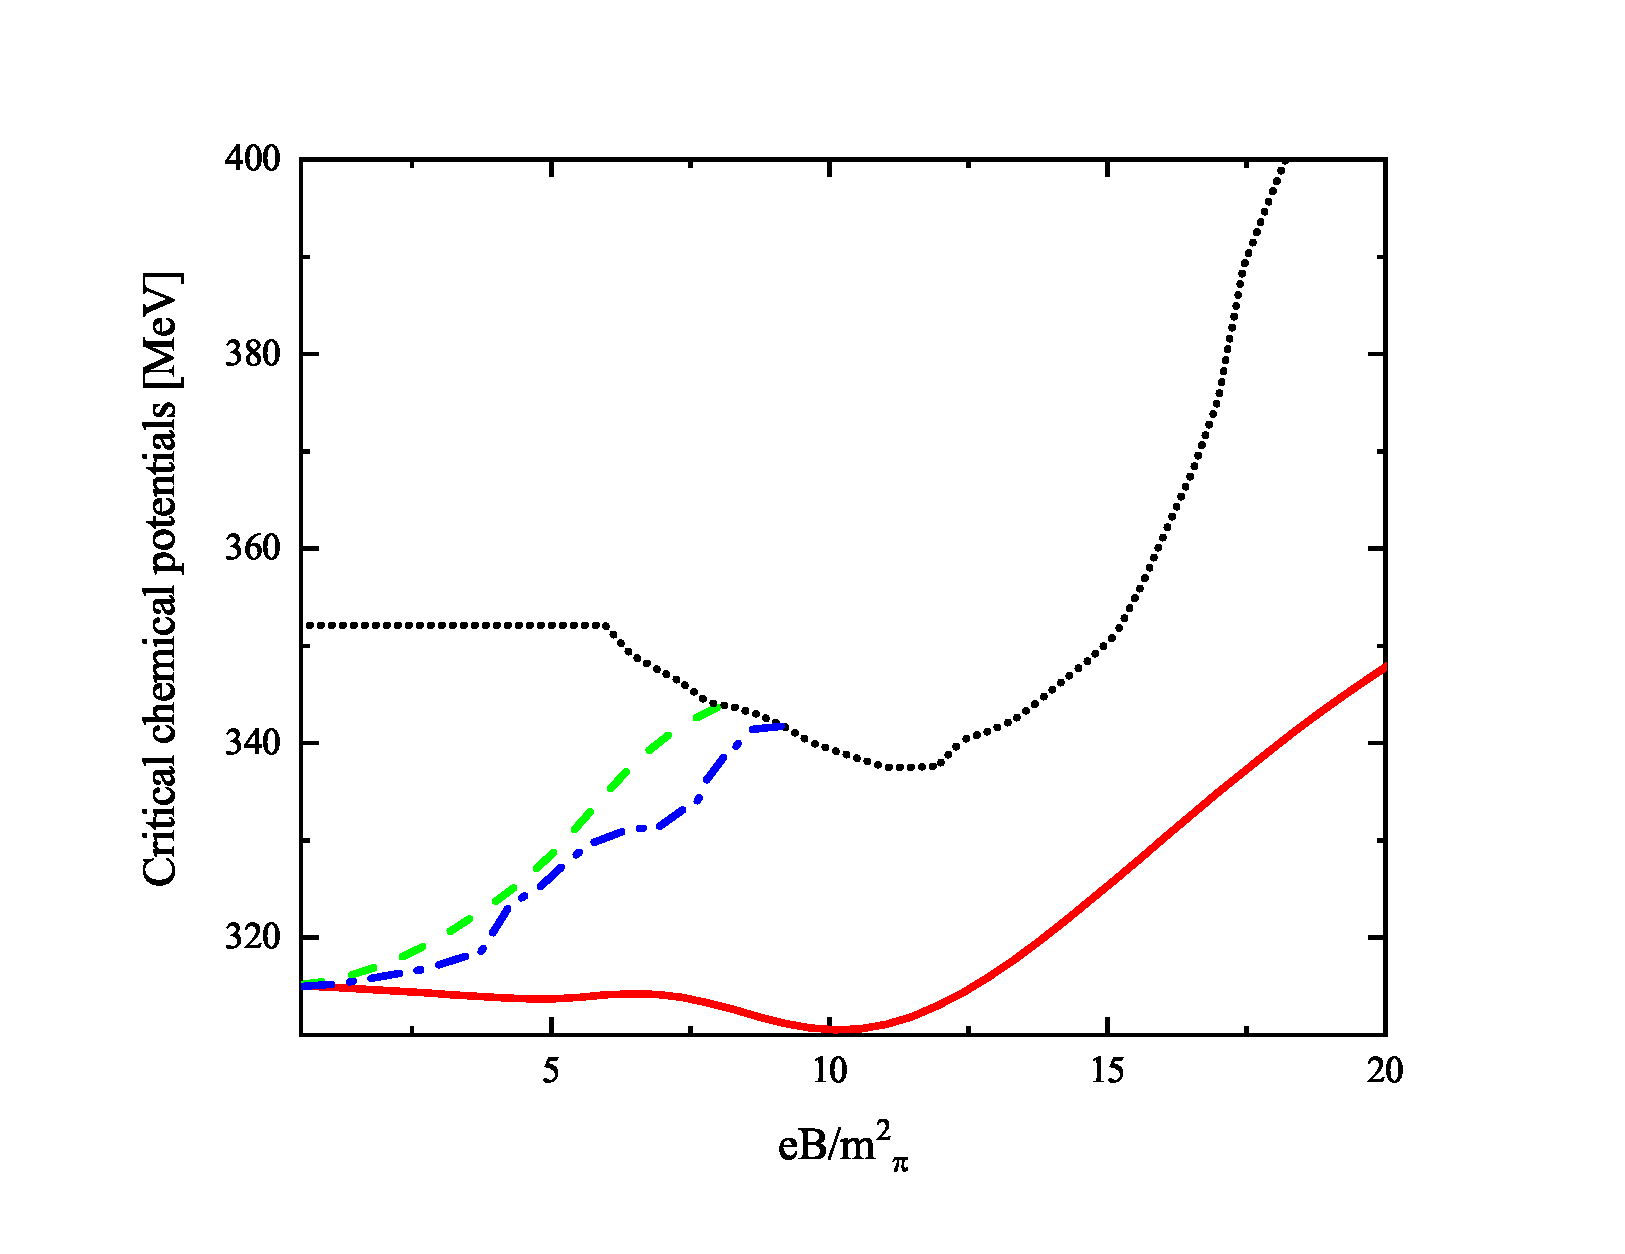
\includegraphics[width=0.6\textwidth]{third.eps}
    \label{fig:thirdpoint}
\end{figure}
With the given model parameters, the critical values for different BEC occurrences
% mentioned in Sec.\ref{sec:2c},  
% $\mu_c^\text{I}$ (solid line) and $\mu_c^\text{II}$ (dashed line) for  $\text{BEC}_\text{I}$  and $\text{BEC}_\text{II}$  occurrences as  functions of the magnetic field
 have been given in Fig.\ref{fig:thirdpoint}.
%are denoted as $\mu_c^\text{I}$ (solid line) and $\mu_c^\text{II}$ (dashed line).
It is clearly shown that with $B$ introduced, $\mu_c^\text{II}$   comes to be larger than $\mu_c^\text{I}$.
%, with introducing magnetic field.
This explains why $\text{BEC}_\text{I}$ phase occurs firstly in the presence of finite magnetic field.
% As $\text{BEC}_\text{I}$ has existed,  $\text{BEC}_\text{II}$ seems to occur sequentially.
%Nevertheless, 
%In Fig.\ref{f3}, it was found that there exist no the   $\text{BEC}_\text{II}$ phase in the QCD phase diagram.
%The reason lies in the fact that 
%not merely $\text{BEC}_\text{I}$ occur at relatively low $\mu$, but also 
As depicted in Fig.\ref{fig:thirdpoint},
$\text{BEC}_\text{II}$ (if exists) undergoes a crossover to the BCS phase at $eB \simeq 8 m_\pi^2$.
Indeed, for intermediate magnetic field, there is the position of the so-called BEC phase.
As depicted in Fig.\ref{fig:thirdpoint}, 
the BEC phase exists until
%the quark chemical potential decided by $\mu=M$ as dot line behaves as critical point for the BEC-BCS crossover.
%At $eB \simeq 8 m_\pi^2$,  $\text{BEC}_\text{II}$ phase disappears since the crossover to BCS phase has happened. In fact,
%there exist no possibility for  the imaginary $\text{BEC}_\text{II}$ phase with zero value of diquark condensate $s_B$, owing to   non-zero value of diquark condensate $s_B$ raises firstly.
%Therefore BEC phase with non-zero value of diquark condensates $s$ and $s_B$ appears in the phase diagram.
 the line of $\mu_c$ meets the line of $\mu_X$ at almost $eB \simeq 9 m_\pi^2$.
Obviously, it   corresponds to the threshold value of magnetic field $eB_{thr}$. This fact could explain the 
result for phase diagram Fig.\ref{f3}.



Moreover,  it is worthy being stressed that various of critical chemical potentials have the different $B$-dependence tendencies.
For $\text{BEC}_\text{II}$ occurrence, $\mu_c^\text{II}$  behaves as an increasing function of $eB$.
Also for BEC occurrence, 
%the value of
 $\mu_c$ is  an almost  monotonic increasing function.
However,  $\mu_c^\text{I}$ is not a monotonic increasing function, but behaves as an evidently decreasing  function
 at $ 6 m_\pi^2 <eB < 10 m_\pi^2$ regime.
Keep in mind that $\mu_c^\text{I}$ can be understood as  the critical end point of chiral phase transition,
therefore the intermediate magnetic field makes   chiral phase transition occur at relatively low chemical potential.
It is totally different from the case  of magnetic catalysis.
% , namely,  has  increasing tendency with magnetic field.
 Such a
phenomenon, inconsistency with magnetic catalysis,  may be regarded as inverse magnetic catalysis (IMC).
Owing to this IMC effect,  $\mu_c^\text{I}$ is always less than the value of BEC-BCS crossover. 
%%
In this sense, the IMC happened in $T=0$ and intermediate value of magnetic field is responsible for the result in phase diagram.

To this end, one may wonder whether or not the IMC effect originates from the oscillation of three gaps.
For $\mu_X$, there exist oscillation behavior.
In our opinion, the oscillation behavior is not main reason for the IMC effect for $\mu^\text{I}_c$.
In other words, the conclusion for IMC would not be invalid even though one may use more reasonable regulator function to
 remove non-physical oscillation. 
This point has been stressed in Ref.\cite{Duarte2015BEC}.

\subsection{Strong  field analysis for  $\text{BEC}_\text{I}$}
\label{sec:3c}

In order to illustrate the meaning of the strong magnetic field in this context,  let us discuss two of extreme conditions.
For the chiral condensate in low energy QCD with only the chiral condensate existed, the dispersion relation  is
$\epsilon^2 = p_3^2 + 2neB + M^2$.
When $eB > M^2$, the Lowest Landau Level (LLL)  works.
%the magnetic effect could not be ignored if the magnetic field scale  reached to $m_\pi^2$.
 A typical example for strong magnetic fields observed in collision experiments,  
 are estimated to have magnitudes of the order $eB \sim 15 m_\pi^2$\cite{V2009ESTIMATE}.
In high density QCD with only diquark-condensate,
the dispersion relation for charged quasiparticles at the Fermi surface is
$\epsilon^2 = (p_3^2 +2neB \pm \mu^2)^2 + \Delta_B^2$.
In contrast,
the relevant scale for the generation of the diquark gaps 
is the energy at Fermi surface, i.e. the chemical potential.
It is logical that once the magnitude of the magnetic field is
comparable to the chemical potential, 
%$\mu^2$ is used as the system of the magnetic  field scale.
As shown in \cite{ferrer2005magnetic}, the value of magnetic field reached to $\mu^2$,
 the difference between $\Delta$ and $\Delta_B$ gaps of the magnetized CFL phase becomes significant and can be treated as strong fields in the magnetized quark matter.
In our context regarding COE of chiral-diquark condensate, our concerned is the quark matter regime with $M= \mu$ (i.e. the density with $\mu_X$).
Therefore the so-called ``strong field" means that $eB > \mu_X^2$, or $M^2$.


 %When the magnitude of magnetic field is sufficiently large
 In this limit, since the LLL works, the system dimension could be reduced to $1+1$ dimension. The summation in Eq.~\eqref{eq:criticalforq} has reduced to only one term.
After such a simplification, the first term  of R.H.S. in Eq.~\eqref{eq:criticalforq} may be rewritten as
\begin{equation}\label{eq:cond2}
 \frac{eB}{ 2\pi^2} \int h_{\Lambda,B}^{n=0}
\frac{ \sqrt{p_3^2 + M^2}}{p_3^2 + M^2 - \mu^2} dp_3.
\end{equation}
By using Eq.~\eqref{eq:cond2}, Eq.~\eqref{eq:criticalforq} can be simplified as
\begin{equation}\label{eq:cond3}
  \frac{1}{H'} = \frac{4}{\pi^2}\int^\Lambda_0 \frac{E}{E^2-\mu^2} p^2 dp 
  + \frac{eB}{2\pi^2} \int^\Lambda_0
  \frac{E}{E^2-\mu^2} dp,
\end{equation}
where the single-particle energy $E= \sqrt{p^2 +M^2}$  and the usual
hard cutoff regularization function has been adopted.

% Note that the magnetic field values considered in the following, $eB =14m_\pi^2$ and $eB =20 m_\pi^2$  are referred to in the literature as strong magnetic fields.
% One one hand, 
% On the other hand, 
% it was found that at the magnetic field region $eB > \mu^2$, 

By using Eq.~\eqref{eq:cond3}, it can be easily found that 
the critical value of  $\mu^{I}_c$ increases with $B$.
%As also shown in Fig.\ref{fig:thirdpoint}, 
%the location of $\mu^{I}_c$ shift  to relatively larger chemical potential 
%with given model parameter. As also depicted in Fig.\ref{fig:thirdpoint}, the value of $\mu_X$ is always larger than that of $\mu^{I}_c$.
%Therefore the  $\text{BEC}_\text{I}$ phase exists still and the location of  $\text{BEC}_\text{I}$ becomes larger with
Of course, this tendency can be found from
the behavior of $\mu^{I}_c$-$B$ function for strong field regime in Fig.\ref{fig:thirdpoint}.
Numerical calculations shows that Eq.~\eqref{eq:cond3} becomes valid
for about $eB > 11 m_\pi^2$ (G), which is the strong field regimes in this context.


%Once the axial anomaly is introduced, 
As stressed above, axial anomaly leads to the additional
 chiral-diquark interplay and makes the diquark coupling become  the effective diquark coupling $H' = H -\frac{1}{4}K'\chi$.
 On the other hand, we will apply Eq.\ref{eq:cond3} to investigate how
 the axial anomaly required for $\text{BEC}_\text{I}$ varies for strong
 magnetic fields.
%This is the essential reason that the axial anomaly raise the COE of chiral and diquark condensates and thus diquark BEC phase occur.
%Therefore, it is necessary to discuss the effect of magnetic field on such an effective diquark coupling.

%As shown  in Eq.~\eqref{eq:cond3}, effective diquark coupling is mainly determined by the value of the effective mass and chemical potential.
%In order to show the magnetic effect, the chemical potential dependence in criterion equation are given at a specific value say, $\mu= 315$ MeV(zero-field).
%As for the effective mass, 
\begin{figure}[h]
  \caption{  The ratio of required effective coupling  for  the diquark $\text{BEC}_\text{I}$ phase transition, with magnetic
  catalysis effect from $M$ (solid line) and without magnetic catalysis effect from $M$ (dashed line). }
  \centering
    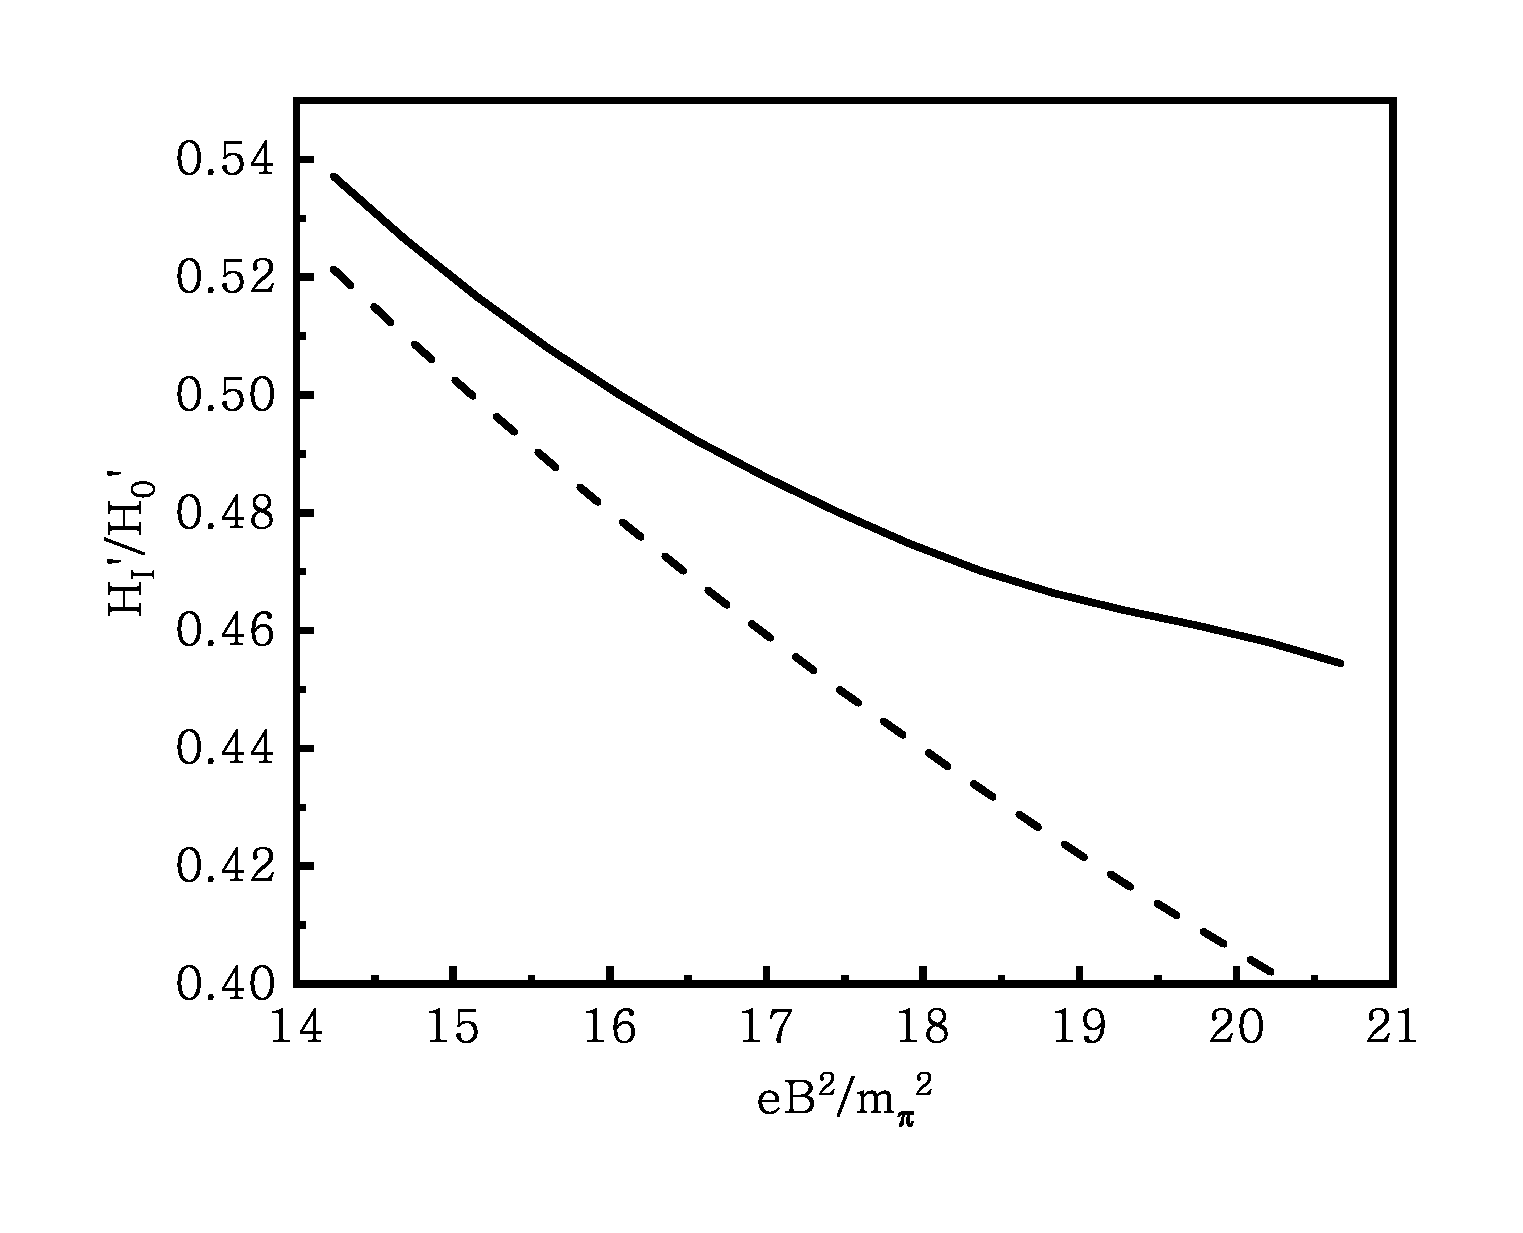
\includegraphics[width=0.5\textwidth]{high.eps}
    \label{fig:h}
\end{figure}

For the  $\text{BEC}_\text{I}$ occurrence, we give the magnetic-field dependence of $H'$  
at a given chemical potential(say $\mu=315$MeV).
%  we can give the magnetic field behavior of $H'$ by
%  incorporating  $M$  into Eq.~\eqref{eq:cond3} through the  single particle energy $E$.
In Fig.\ref{fig:h}, we have normalized the diquark effective coupling $H'$
with respect to $H'_0$ obtained at zero-field limit.
As depicted in Fig.\ref{fig:h}, $H'$ (the solid line)
manifest a monotonic decreasing function.
This decreasing tendency indicates that strong fields facilitate the occurrence of $\text{BEC}_\text{I}$, which can be mainly attributed to
an explicit coupling to $eB$ (i.e., the second term of Eq.~\eqref{eq:cond3}).
%In fact, the behavior of $H'_{I}$ depends on the effect for  $eB$ relevant term as well as magnetic catalysis effect  from
% the effective mass $M$.
Besides, the strong field result of $H'$ also has an implicit $B$-dependence of $E$, exactly the dependence of $M$.
Interestingly, $B$-dependence of M represents 
a monotonic increasing function (i.e., magnetic catalysis 
\cite{Gusynin1994Dimensional,Miransky2012Catalysis}).
If neglecting this MC (i.e., assuming $M$ unchanged), $H'$ as a function of $eB$ displays a  more obvious decreasing function (shown  in Fig.\ref{fig:h}).
It is clear in Fig.\ref{fig:h} that the $B$-dependence of $H'$ 
%indicates that the tendency for the effective coupling $H'_{I}$
is partially compensated by the magnetic effect.





%In order to remove the magnetic effect from $M$, our discussions are organized by the following steps. As the first step, we assume that the effective   mass $M$ keeps unchanged with magnetic field. Then  we consider $B$ dependence of $M$ and turn to give a full analysis of the $H'$ behavior.
%It is worthy being stressed that for our concerned $\text{BEC}_\text{I}$ occurrence, the effective mass only depends on the chiral-related parameter $G$ and $K$ and thus its variation with $B$ can be determined completely, even if the effective coupling $H'$ varies.








%As the effective mass is assumed to be unchanged, it is easy to found that solid line is an obviously
%monotonic decreasing function of $B$ field. 
%Note that, this is different from Fig.\ref{fig:thirdpoint}, where the value of $M$ is not constraint like this case.
%The decreasing behavior as function of strong magnetic field indicates that strong fields facilitate  $\text{BEC}_\text{I}$ occurrence.

%Once magnetic effect for chiral condensate is included, as shown by the solid line, the effective coupling behavior manifest a monotonic decreasing function.
%With increasing magnetic field, the $\text{BEC}_\text{I}$ phase not only remain valid, more importantly, its occurrence become possible even if the axial-anomaly induced interplay is suppressed relatively.
%It implies that the strong field facilitates the $\text{BEC}_\text{I}$ occurrence originated by the chiral-diquark condensate interplay.


\begin{figure}[h]
\caption{  The ratio of  coupling $K'/K$ as  function of chemical potential at strong magnetic field.}
\centering
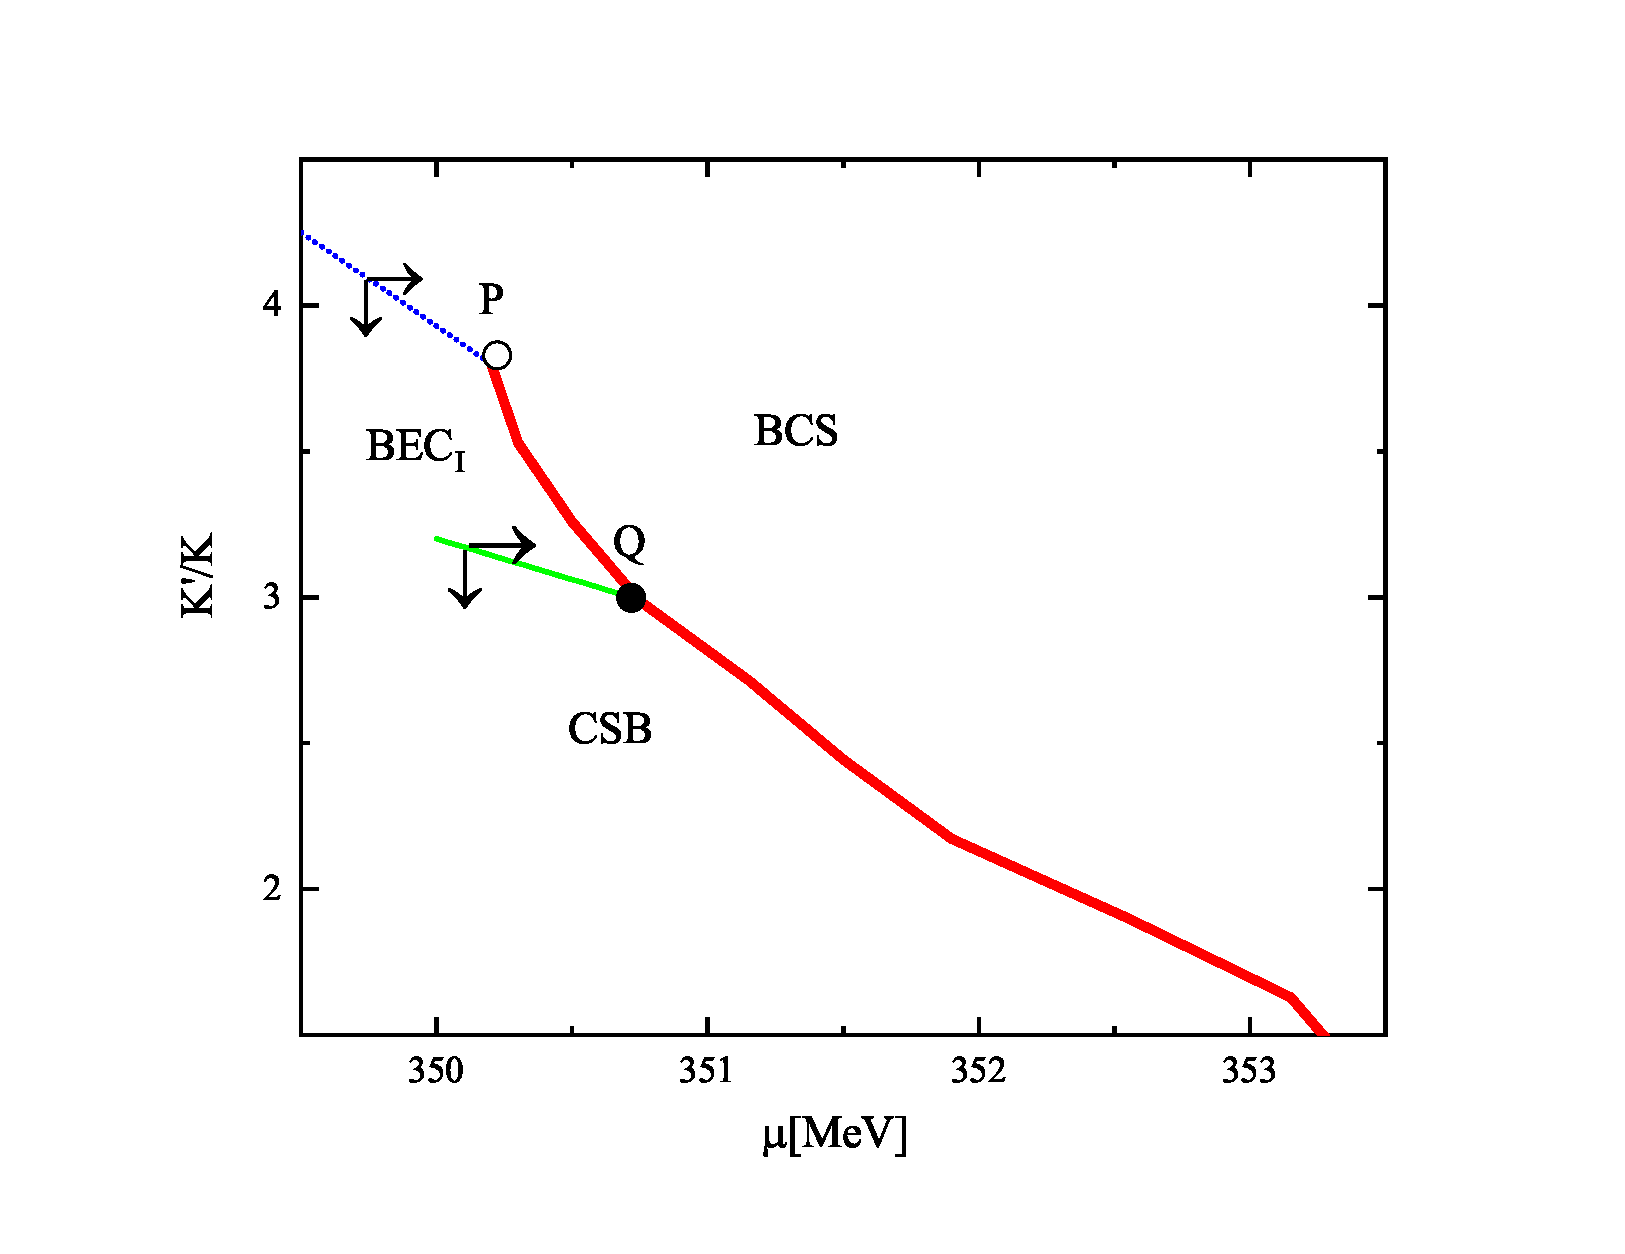
\includegraphics[width=0.6\textwidth]{kmu.eps}
\label{fig:kmu}
\end{figure}

Finally let's turn to discuss the $B$-dependence for chiral-diquark coupling $K'$ qualitatively.
Fig.\ref{fig:kmu} shows the phase diagram in the $\mu$-$K'$ plane for strong magnetic field.
 As shown in Fig.\ref{fig:kmu}, for small $K'$, the phase diagram has a chiral symmetry broken (CSB) region and a BCS region, divided by
 the first-order phase transition line ( solid line).
  For sufficiently large value of $K'$ compared with coupling $K$,
  $\text{BEC}_\text{I}$ as coexistence of chiral condensate $\chi$ and diquark condensate $s_B$ appears across a second-order phase transition (solid line) from the CSB phase.
  For strong field regime, there exist only $\text{BEC}_\text{I}$  and BEC-BCS crossover.
 And the line of  BEC-BCS crossover joint the line of first-order transition line at point $P$.
 Point Q can be treated as the critical end point for chiral phase transition, since the parameter $\chi$ is continuity.
As for point $P$, it represents the transition between  $\text{BEC}_\text{I}$ and BEC-BCS crossover, not a critical end point being different from point $Q$.
For somewhat smaller $K'$, a novel first-order transition appears between $P$ and $Q$.
 %Then the chiral phase transition has returned to a first-order transition in point $Q$. 
With increasing  magnetic field, the line of $\text{BEC}_\text{I}$ as well as  BEC-BCS crossover
shift to  relatively higher chemical potential in  a given value of $K'$.
Physically, it originates from  the MC effect  on   $\text{BEC}_\text{I}$ as well as  BEC-BCS crossover.
If restricting to a given value of $\mu$ ,
as shown in Fig.\ref{fig:kmu}, the line of $\text{BEC}_\text{I}$ as well as  BEC-BCS crossover move to a lower value of $K'$.
This conclusion is equivalent with the  results shown in Fig.\ref{fig:h}.


\section{Conclusion and discussions}

By incorporating the magnetized CFL matter into  a modified three-flavor NJL phenomenological model,
we have investigated the coexistence of chiral condensate and diquark condensate and the critical phenomena at $T=0$.
Based on the rotated electromagnetic mechanism in CFL matter, diquark condensate is split into two species, $s$ and $s_B$.
According to this fact, we have derived the NJL formalism of magnetized CFL matter with axial anomaly.

Introducing axial anomaly  has changed the COE phase structure and the critical phenomena previously predicted in Ref.\cite{abuki2010nambu}.
%Different from the zero field results that the coexistence region  contains a diquark
%BEC phase,  splitting of the Bose Einstein Condensed phase was found at intermediate magnetic regime.
%More precisely, $\text{BEC}_\text{I}$  
%(with $s_B \neq 0$, $s = 0$,$\chi \neq 0$)
%appears first,  BEC
%( with $s \neq 0 $, $s_B \neq 0$ and $\chi \neq 0$)
%raises as follows.
For the strong fields regime,  BEC vanishes and
$\text{BEC}_\text{I}$  occupies the COE phase completely.
In the absence of a magnetic field, three-flavor massless quark matter at high baryonic density is in the energetically favored CFL phase. There, the diquark condensates lock the color and flavor transformations, breaking both symmetries. The symmetry breaking pattern in the CFL phase is
 $SU(3)_C \times SU(3)_L \times SU(3)_R \times U(1)_B \rightarrow SU(3)_{C+L+R}$.
For sufficiently strong magnetic fields, in the magnitized CFL phase the symmetry breaking pattern becomes
$SU(3)_C \times SU(2)_L \times SU(2)_R \times U(1)_B \times U(1)_A \rightarrow  SU(2)_{C+L+R}$\cite{ferrer2006color}.
Physically, for our situation, it might be related with the magnetic field induced  violation of color flavor locked symmetry patterns.
For weak field, CFL symmetry is sightly violated.
The splitting of diquark condensate leads to the seperation of COE, i.e., BEC$_\text{I}$ and BEC.
In this sense, critical phenomena have no essential difference from that of the zero field case.
For larger magnitude of $B$ field, the symmetry breaking becomes obvious.
Because of enhanced magnetic effects on BEC$_\text{I}$ occurrence (see Sec.\ref{sec:3b} for details),
only BEC$_\text{I}$  survive in the COE region.
since  disappears from the phase diagram, 
there exists no longer continuity  between chiral broken phase in low chemical potential and  CFL phase in high temperature.
Even though the axial anomaly interplay is introduced, thus, the critical phenomena predicted in zero field is difficult to realized.


% As known that the BCS phase of magnetized CFL matter have been devoted sufficient researches.
% Different from previous work, we focus on the critical phenomena happened in COE regime.
% The splitting of BEC phase was observed and the specific $\text{BEC}_\text{I}$ phase was firstly proposed in our work.
% The splitting of Bose Einstein Condensed phase represents the magnetic-field induced
% violation of color-flavor symmetry.
% The vanishing behavior for BEC phase indicates that magnetic field totally
% destroys the critical phenomena in the COE regime.
%Within the model with axial anomaly, the nonzero magnetic background is stressed to play its key role on the coexistence and low-temperature critical phenomena.

% Then we have investigated the underling mechanism by deriving the criterion condition for  $\text{BEC}_\text{I}$ and  $\text{BEC}_\text{II}$  occurrences.
For the intermediate magnetic fields, say $eB < 10m_\pi^2$, the critical value of $\mu^{I}_c$ as functions of $eB$
 has a decreasing tendency.
 It reflects that non-vanishing magnetic fields facilitate the Bose Einstein condensation of $s_B$,
 since the charged quarks becomes involved to $eB$ directly.
 Noticing that $\mu^{I}_c$ behaves as the critical end point of chiral transition, more importantly, the tendency can be understood as IMC, i.e.,
 the critical chemical potential for chiral phase transition shifts to a lower value with increasing magnetic field.
In zero temperature QCD, the IMC phenomenon has already been pointed out in Ref.\cite{Duarte2015BEC}.
There, the diquark BEC phase in two-color and two-flavor NJL model has some similar details with  $\text{BEC}_\text{I}$ discussed in the present work.
 In this sense, our result of IMC effect is not a strange phenomenon, and maybe a general property in zero-temperature QCD physics.




 For strong magnetic field, say $eB > 15m_\pi^2$,
 % the $\text{BEC}_\text{I}$ occurrence has some of significant features.
  %since analysis discussion is available.
%   with the given model parameters, the $B$-dependence of $\mu_c^{I}$ is studied.
%  As shown in Fig.\ref{fig:thirdpoint}, 
 the location of $\text{BEC}_\text{I}$ is found at relatively large chemical potential.
 %Therefore, strong field make it possible that the coexistence of $\chi$ and $s_B$ appears at a relatively high density.
Also, the effective coupling $H'_{I}$ is observed to be relatively small for strong field.
% Because of Eq.~\eqref{eq:effectivecoupling}, it is clear that the strength of the relevant axial anomaly parameter $K'$ decreases with magnetic field.
 %Therefore, 
 As discussed in Sec.\ref{sec:3c}, 
 such tendencies preserves with increasing magnetic field.
 %it is possible that strong fields makes it possible that the diquark-chiral coexistence appears when a relatively small axial anomaly coupling is chose.
It is known that the QCD axial anomaly caused by instanton effects would be suppressed at high densities\cite{T2002Instanton,R2000High}.
Therefore, it is reasonable to expect that the situation with strong field corresponds to a more realistic physical environment.
If magnetars have color-superconducting cores, it is very likely that the present-discussed $\text{BEC}_\text{I}$ and the corresponding
coexistence with chiral and diquark condensate 
%critical phenomena
provide key information for the observation of magnetars
%and understanding physics of magnetars.

Exploring the critical phenomena in realistic QCD environment is 
a important task for phenomenological models and lattice QCD simulations.
The present work have extended the analysis of Ref.\cite{abuki2010nambu} by including additional magnetic effect. To make our numerical results  more 
realistic, there are many other aspects have not yet been considered.
For a three-flavor NJL model with including quark bare masses, Ref.\cite{basler2010role} shows that 2SC pairing could be favored owe to spontaneous flavor-symmetry breaking caused by the axial anomaly and this would lead to a rich phase structure.
It would be interesting to  investigate open problems include whether the 2SC pairing  would survive in COE region,
when the additional magnetic fields are turned on, and how the  phase 
structure changes with magnetic fields.

It is also important for us to make our numerical results more
realistic by including Polyakov loop term describing the deconfinement transition.
For a three-flavor NJL model with Polyakov loop, it was shown in Ref.\cite{Powell2013Asymmetric}
that Polyakov loop could give rise to an ACFL phase without a local 
color neutrality constraint. There remain open questions of whether
ACFL phase would survive in the COE region with the magnetic field included, and how the QCD phase diagram changes with different magnitude values of magnetic fields.

The existence of kaon condensate in the CFL phase  is another important  aspects to simulate realistic QCD environment\cite{Sch2000Kaon}.
This might make the COE region in the QCD phase diagram more complicated. 
Note that we have ignored the color neutrality by restricting ourselves to one single chemical potential.
In general, we believe that these problems listed above might be important and  worthful to investigate in the future.
%\bibliographystyle{apsrev4}
\bibliographystyle{unsrtnat}
\bibliography{bibfile}

\end{document}












